\documentclass[preprint,12pt]{elsarticle}
% Supplementary Material -- figures/tables generated from the original records (see *_PROVENANCE*.json)
\usepackage{amsmath,amssymb}
\usepackage{graphicx}
\usepackage{booktabs,multirow,array}
\usepackage[hidelinks]{hyperref}
\graphicspath{{./}}
\newcommand{\tabdir}{}
\renewcommand{\Pr}{\operatorname{P}}
\newcommand{\Bin}{\operatorname{Bin}}
\renewcommand{\thefigure}{S\arabic{figure}}
\renewcommand{\thetable}{S\arabic{table}}
\renewcommand{\theequation}{S\arabic{equation}}
\renewcommand{\thesection}{S\arabic{section}}
\journal{Robotics and Autonomous Systems}

\begin{document}

\begin{frontmatter}
\title{Supplementary Material for ``When Recovery Hurts: Separating Rescue from Harm in an Observation-Only Recovery Intervention for a Frozen Visuomotor Policy''}
\author{[Author name to confirm]}
\end{frontmatter}

This document gives the statistical details, the development history that motivated the controller, its constants, the abstention counts of every stage, the full record of the harm case, the physics-validity measurements, the recount, and the deviations and environment of every run. Figure and table numbers prefixed with S refer to this document; others refer to the main text.

%% -----------------------------------------------------------------------------------------------
\section{Statistical details}\label{sec:s-stats}

\paragraph{Sampling model} Scene seeds of a split are distinct integers; each seed determines the cube placements through the simulator's reset. We treat the scenes of a split as independent draws from the scene distribution $\mathcal{D}$ restricted to that split and assume that the policy's behaviour depends on the seed only through the scene (the policy's sampling noise is fixed per scene and identical for all branches). A placement check confirmed that no calibration or test scene repeats a placement of any earlier scene.

\paragraph{Conditional binomial argument for the certificate} Let $(Y_0^{(i)},Y_g^{(i)})$, $i=1,\dots,n$, be i.i.d. Write $S=\{i: Y_0^{(i)}=1\}$ and $n_+=|S|$. Given $S$, the variables $(1-Y_g^{(i)})_{i\in S}$ are i.i.d.\ Bernoulli with parameter $h(g)=\Pr(Y_g=0\mid Y_0=1)$, because the pairs are independent across scenes and each pair's conditional law depends only on its own $Y_0$. Hence $k=\sum_{i\in S}(1-Y_g^{(i)})\sim\Bin(n_+,h)$ conditionally on $S$, and for every $h>\varepsilon$
\begin{equation}
\Pr\bigl(p_{\mathrm{harm}}\le a \bigm| S\bigr)\le a\qquad\text{for all } a\in[0,1],
\end{equation}
since $p_{\mathrm{harm}}=F_{\Bin(n_+,\varepsilon)}(k)$ is a valid p-value for $H_0: h>\varepsilon$ (also at $h=\varepsilon$) and the binomial distribution function is decreasing in $h$. Averaging over $S$ gives the unconditional statement. Holm's step-down procedure over the two policies controls the family-wise error at $\delta$ without assumptions on the dependence between the two p-values.

\paragraph{Exact paired efficacy test} With $b$ rescues and $c$ harms, $d=b+c$, the conditional law of $b$ given $d$ is $\Bin(d,\theta)$ with $\theta=\Pr(\text{rescue})/(\Pr(\text{rescue})+\Pr(\text{harm}))$. The null hypothesis of no improvement is $\theta\le1/2$, and $p_{\mathrm{eff}}=\Pr(\Bin(d,1/2)\ge b)$. For $b=29,c=0$, $p=2^{-29}=1.86\times10^{-9}$; for $b=27,c=1$, $p=28\cdot2^{-28}+2^{-28}=1.08\times10^{-7}$.

\paragraph{Intersection--union test for $H_{\mathrm{mem}}$} The memory hypothesis requires an improvement for both policies. The intersection--union test rejects the union of the two policy-level nulls when both are rejected at the same level; its p-value is the maximum of the two, $\max(0.0059,0.0078)=0.0078$.

\paragraph{Post hoc descriptive quantities} Table~\ref{tab:s-desc} adds one-sided 95\% Clopper--Pearson upper bounds of the conditional harm and paired bootstrap intervals (20,000 resamples of scenes, percentile method, random seed 20261123) of the success difference. They were computed after the confirmatory stages, change no pre-registered decision, and are reported for orientation only.

\begin{table}[!htbp]
\centering\footnotesize
\caption{Post hoc descriptive quantities for calibration and Final Test. ``Moved among $Y_0{=}1$'': baseline successes in which V2 made a move.}\label{tab:s-desc}
\resizebox{\linewidth}{!}{\input{\tabdir TS2_descriptive_posthoc.tex}}
\end{table}

\paragraph{Power considerations} With $\varepsilon=0.05$, the certificate passes at the Holm level $0.025$ for up to 8 harms ($n_+=337$) or 9 harms ($n_+=348$), and at level $0.05$ for up to 10 harms (Eq.~(3) of the main text); the observed 1 and 0 harms are far from that boundary.

%% -----------------------------------------------------------------------------------------------
\section{Development history that motivated V2}\label{sec:s-history}

All of the following are development results on scene sets that were used once and are not part of calibration or test.
\begin{enumerate}
\item \textbf{Failure diagnostic} (seeds 50600--50699, policy seed 1, no intervention): 79 successes and 21 failures. Read after the run, the 14 failures that released the cube over the target let go of it 1.7--4.7\,cm off-centre, successes at most 2.3\,cm; up to 1.5\,cm offset, 62 episodes had 0 failures, above 2.5\,cm, 8 had 8 failures.
\item \textbf{Oracle centring pilot} (seeds 50700--50799): no intervention 82, 5\,cm retreat 73, matched hold 82, oracle centring 92; centring against no intervention: 10 rescues, 0 harms; the retreat turned 14 successes into failures. Interrupting, waiting and re-planning (the matched hold) did not explain the gain.
\item \textbf{Vision-CENTER V1} (wrist camera only, no memory; seeds 50800--50899): C0 91, V1 92, oracle 96; V1 recovered 1 of 5 oracle rescues and missed 4 by abstaining because the target was hidden (2) or the held cube was not fitted (2). This motivated the memory of V2.
\item \textbf{V2 development} (seeds 50900--51099 and earlier used scenes; policy seed 1) and the pre-registered C1 stage reported in the main text. Nothing was adapted to policy seed 2.
\end{enumerate}

%% -----------------------------------------------------------------------------------------------
\section{Controller constants and decisions}\label{sec:s-constants}

\begin{table}[!htbp]
\centering\footnotesize
\caption{Constants of Vision-CENTER V2 (frozen before calibration; source \texttt{src/hci/vision\_center\_v2.py}, \texttt{vision\_center.py}, \texttt{recovery\_v1\_oracle.py}).}\label{tab:s-const}
\begin{tabular}{p{0.45\linewidth}r}
\toprule
Quantity & Value\\
\midrule
Trigger: open command after at least $n$ close commands & $n=3$\\
Trigger: finger opening (sum of joints) & 0.02--0.06\,m\\
Act if estimated offset $\ge$ & 15\,mm\\
\ldots{} and offset minus reading bound $\ge$ & 10\,mm\\
Reading bound: wrist-camera fit / base camera / hold fit & 2 / 5 / 2\,mm\\
Extra bound after a near pass of the gripper & 5\,mm\\
Memory confirmations before use ($m$) & 3 (single-frame variant: 1)\\
Hold memory dropped if finger opening changes by more than & 1\,mm\\
Hold refit interval while closed & every 4 steps\\
Minimum carried height of the held cube centre & 58\,mm\\
Minimum steps left in the episode & 20\\
Command per step / target cap / maximum steps & 5\,mm / 30\,mm / 12\\
Stop when residual offset $\le$ (frame / memory target) & 10 / 5\,mm\\
Stop if target jumps or held cube slips by more than & 3\,mm\\
Side-contact rule: centre distance at least & 40\,mm (+ bound)\\
\ldots{} and held-cube bottom above target top by at least & 3\,mm\\
\bottomrule
\end{tabular}
\end{table}

\begin{table}[!htbp]
\centering\footnotesize
\caption{V2 decision at the trigger in every scene of every stage (raw scene records). s1, s2: policy seeds.}\label{tab:s-dec}
\resizebox{\linewidth}{!}{\input{\tabdir TS1_decisions_by_stage.tex}}
\end{table}

\begin{figure}[!htbp]
\centering
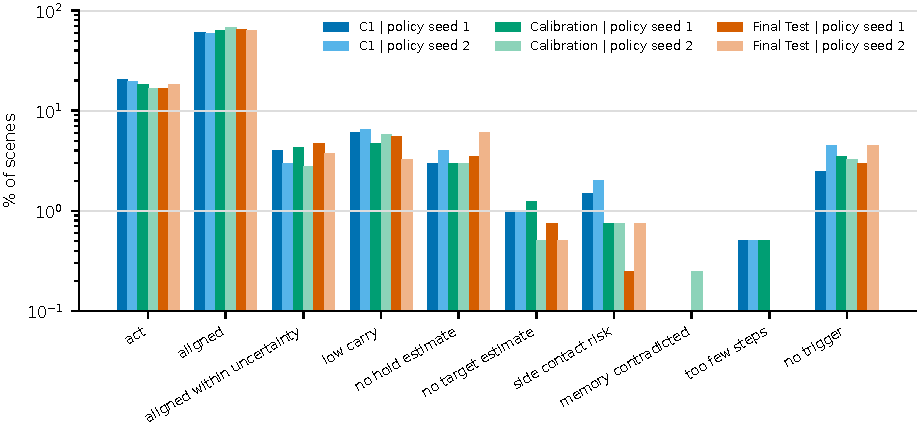
\includegraphics[width=\linewidth]{S2_decisions_by_stage.pdf}
\caption{Share of each V2 decision per stage and policy (log scale). The proportions are stable from development to calibration and test: V2 acts in 16--21\% of scenes, and about two thirds of scenes are already aligned at the trigger.}\label{fig:s-dec}
\end{figure}

%% -----------------------------------------------------------------------------------------------
\section{The development harm case 51157 in full}\label{sec:s-51157}

\begin{figure}[!htbp]
\centering
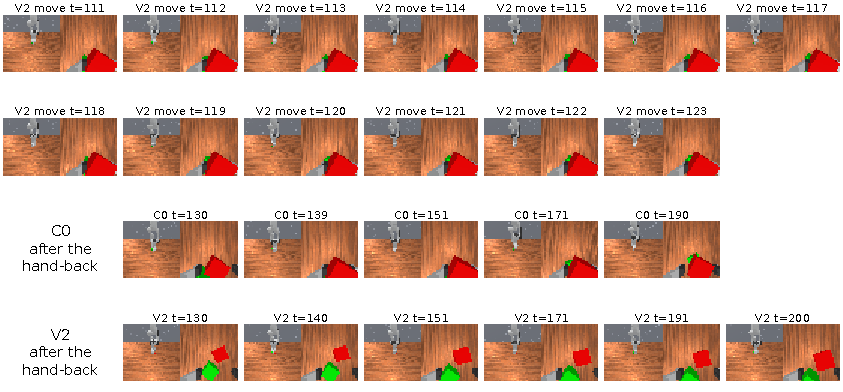
\includegraphics[width=\linewidth]{S1_frames_51157.pdf}
\caption{Scene 51157, policy seed 1. Rows 1--2: all 13 stored frames of the V2 move (trigger at step 111). Rows 3--4: frames after the hand-back for C0 and V2. Each frame is base camera (left) and wrist camera (right), unprocessed. C0 regrasps the dropped cube and succeeds at step 190; with V2 the cube lies beside the target and the episode ends at the horizon.}\label{fig:s-frames}
\end{figure}

\begin{figure}[!htbp]
\centering
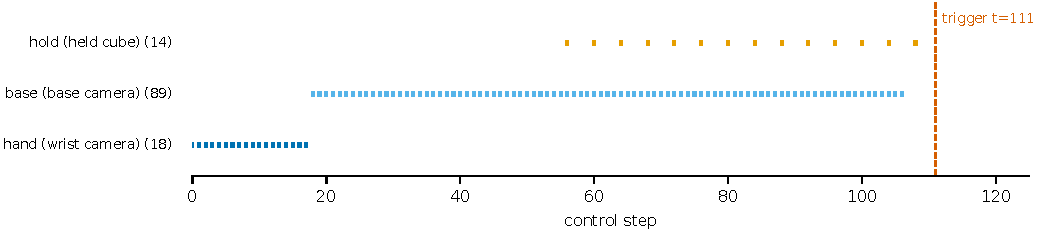
\includegraphics[width=\linewidth]{S3_memory_timeline_51157.pdf}
\caption{Accepted memory observations before the trigger in scene 51157 (hand 18, base 89, hold 14; no conflict). The target was seen by the wrist camera early in the episode and by the base camera until step 106.}\label{fig:s-mem}
\end{figure}

\paragraph{Record} Trigger at step 111 with a 58-step closing run and finger opening 48.8\,mm. True offset 54.6\,mm, estimated 54.7\,mm (reading bound 9\,mm, error 0.15\,mm). V2 acted for 12 steps; the TCP moved 24.3\,mm horizontally and 1.0\,mm down, the held cube 24.2\,mm; cube B did not move; the grasp was kept. The residual offset was 30.4\,mm. C0 reached success at step 190; V2 ran to the 200-step horizon.

%% -----------------------------------------------------------------------------------------------
\section{Commanded versus actual motion (Check 4)}\label{sec:s-check4}

Check 4 was declared before the C1 run: every move step must have direction cosine $\ge0.9$ between actual and commanded horizontal TCP displacement and progress $\ge0.2$\,mm along the command. V2 failed it in 9 of 41 (seed 1) and 5 of 39 (seed 2) moves. Three independent computations (the audit CSV, re-running the audit function, an independent recomputation) agreed on all 715 acted branches. In every failing move of every arm (110 moves), only the first step failed; a post hoc check of steps 2 and later passed in all 715 moves. The first-step failures had no robot--target or robot--table impulse in the contact list, and the V2 failures had a smaller cosine between the first command and the motion before the trigger (median $-0.57$ vs $0.66$ for passing moves), consistent with the arm still moving with the policy's previous command.

%% -----------------------------------------------------------------------------------------------
\section{Physics-validity measurements}\label{sec:s-physics}

\paragraph{S6 definition} For each contact pair that PhysX lists (pairs whose shapes are within the sum of their contact offsets, 0.02\,m each), the logged separation is compared with the signed gap reconstructed from the logged body poses and collision shapes. A row fails when the two differ by more than 1\,mm. Over the development record 54,267 of 580,539 rows fail (9.3\%); per pair kind see Fig.~7a of the main text.

\paragraph{Independent reconstruction} A second, independent reconstruction on a subset agreed with the first within $10^{-12}$\,mm for all kinds except cube B--table ($4\times10^{-6}$\,mm); the disagreement is therefore between PhysX and the poses, not between our two reconstructions.

\paragraph{Static known geometry} 59 static cases (aligned, rotated, edge and vertex configurations of two boxes; gaps from $-3$ to $40$\,mm) were simulated for one step. In the 56 cases with listed contact points, the PhysX separation equals the analytic gap \emph{before} the last sub-step within 0.05\,mm.

\paragraph{Sub-step logging (B4)} Logging every one of the five physics sub-steps per control step on 11 used scene-runs gave 56,558 separated listed pairs at the last sub-step. Compared with the pose after the step, 5,181 exceed 1\,mm (median 0.044\,mm); compared with the pose before the last sub-step, 1,874 (median $2\times10^{-5}$\,mm). By relative speed: below 1\,mm/s 137 $\to$ 137; 1--10\,mm/s 690 $\to$ 681; 10--100\,mm/s 918 $\to$ 910; above 100\,mm/s 3,436 $\to$ 146. The residual 1,874 rows are zero-impulse proximity pairs of a finger box and a cube in which PhysX reports a larger separation than the reconstruction. Shape-index mismatch (17 of 45,645) and static edge geometry (20 dedicated cases, zero difference to GJK) were excluded. Note that this run's traces differ from the original development traces (host difference), so B4 describes the simulator on the calibration host.

\paragraph{Hull sensitivity} Replacing each logged link mesh by the convex hull of its vertices (volume excess at most 0.29\%) and recomputing S4 and S5 on all 3,874 branches changed no status and no S4 distance.

%% -----------------------------------------------------------------------------------------------
\section{Generalisation details}\label{sec:s-gen}

The PlainConv policy is the project's earlier diffusion policy with the original small, non-pretrained convolutional encoder (500 demonstrations, 100,000 updates; qualification 37/100). V2 was applied without any change on new development seeds 51300--51499 (0 identical placements). One test was pre-declared: $H_{\mathrm{arch}}$, V2 against C0, exact one-sided paired test: 37 vs 2, $p=1.4\times10^{-9}$. V2 recovered 37 of the 45 oracle rescues; V2 against single frame was 8 vs 0 (descriptive).

%% -----------------------------------------------------------------------------------------------
\section{Recount and provenance}\label{sec:s-recount}

Every headline number was recomputed from the raw scene records by \texttt{figures/source\_code/recount\_all.py}. Before counting, the SHA-256 of each trajectory file was checked against the hash stored in its scene record, and the absence of error records was asserted. Two implementations were compared: (A) the project's analysis functions and (B) a hand-written count with \texttt{scipy.stats.binom} and a hand-written Holm procedure. All counts were identical and all p-values agreed within $10^{-12}$. The B3 counts also matched the server analysis. Figures and tables are generated by scripts that store the SHA-256 of every input and output.

\begin{table}[!htbp]
\centering\footnotesize
\caption{Frozen artefacts.}\label{tab:s-hash}
\begin{tabular}{ll}
\toprule
Artefact & SHA-256 (prefix)\\
\midrule
C1 development plan & \texttt{6b3f04fe\ldots}\\
Amendment 017 (confirmatory design) & \texttt{b8fd6324\ldots}\\
Calibration manifest (28 files) & \texttt{01b70a06\ldots}\\
Final Test manifest (42 files) & \texttt{94c5a591\ldots}\\
\bottomrule
\end{tabular}
\end{table}

%% -----------------------------------------------------------------------------------------------
\section{Environment, deviations and cost}\label{sec:s-env}

\paragraph{Software} ManiSkill 3.0.1 at commit \texttt{a4a4f92}, SAPIEN 3.0.3, PhysX CPU, Python 3.10, single environment; full package list frozen with the manifests.

\paragraph{Hosts} Development (C1): NVIDIA driver 550.120, Intel i7-13700K. Calibration, Final Test and B3/B4: RTX 4090, driver 595.99.02, Intel i7-10700. Rendering and therefore policy actions differ between the drivers; outcome differences between hosts were found in 16 of 300 scenes of an earlier stage and in 6 of 11 selected diagnostic scenes.

\paragraph{Deviation} The calibration design required a smoke run to reproduce the C1 records bit for bit. It reproduced none of 6 scene-runs (trunks differ; the C0 outcome of 51157 changed), but it reproduced the unchanged C1 collector on the same host exactly. The decision to proceed with a fixed host type was committed before the first calibration rollout; it was taken by the AI agent that ran the experiment, was not separately approved in advance, and was reviewed by the author afterwards, who takes responsibility for it. Nothing about the candidate, policies, levels, tests or rules changed.

\paragraph{Execution notes} The calibration pass of policy seed 2 was started as a separate parallel process for speed; the original chain's seed-2 step was therefore refused as ``already exists'' (exit code 1), as designed, and the analysis ran as a separate step. The first B4 attempt did not log (the simulator rebuilds its scene at reset) and is kept as a failed try. The Final Test ran once; nothing was changed or re-run after it.

\paragraph{Cost} Rented GPU time: calibration US\$1.75, B3 US\$0.67, B4 US\$0.32, Final Test US\$2.13.

\end{document}
